\documentclass[11pt]{article}

% ==== Paquetes ====
\usepackage[utf8]{inputenc}
\usepackage[spanish]{babel}
\usepackage{amsmath, amssymb, amsfonts, siunitx}
\usepackage{graphicx}
\usepackage{float}
\usepackage{pdfpages}
\usepackage{listings} % Para código
\usepackage{xcolor}
\usepackage{hyperref}
\usepackage{caption}
\usepackage{subcaption}
\usepackage{geometry}
\usepackage{tikz}

\geometry{margin=2.5cm}

% ==== Configuración de listings (para código) ====
\lstset{
    language=Python,
    basicstyle=\ttfamily\small,
    keywordstyle=\color{blue},
    stringstyle=\color{green!50!black},
    commentstyle=\color{red!50!brown},
    showstringspaces=false,
    frame=single,
    breaklines=true,
    numbers=left,
    numberstyle=\tiny\color{gray},
    tabsize=4
}

% ==== Datos de la tarea ====
\title{IEE3584 - Comunicaciones inalámbricas \\
Tarea 1}
\author{Nicolás Seguel}
\date{Agosto 2025}

\begin{document}
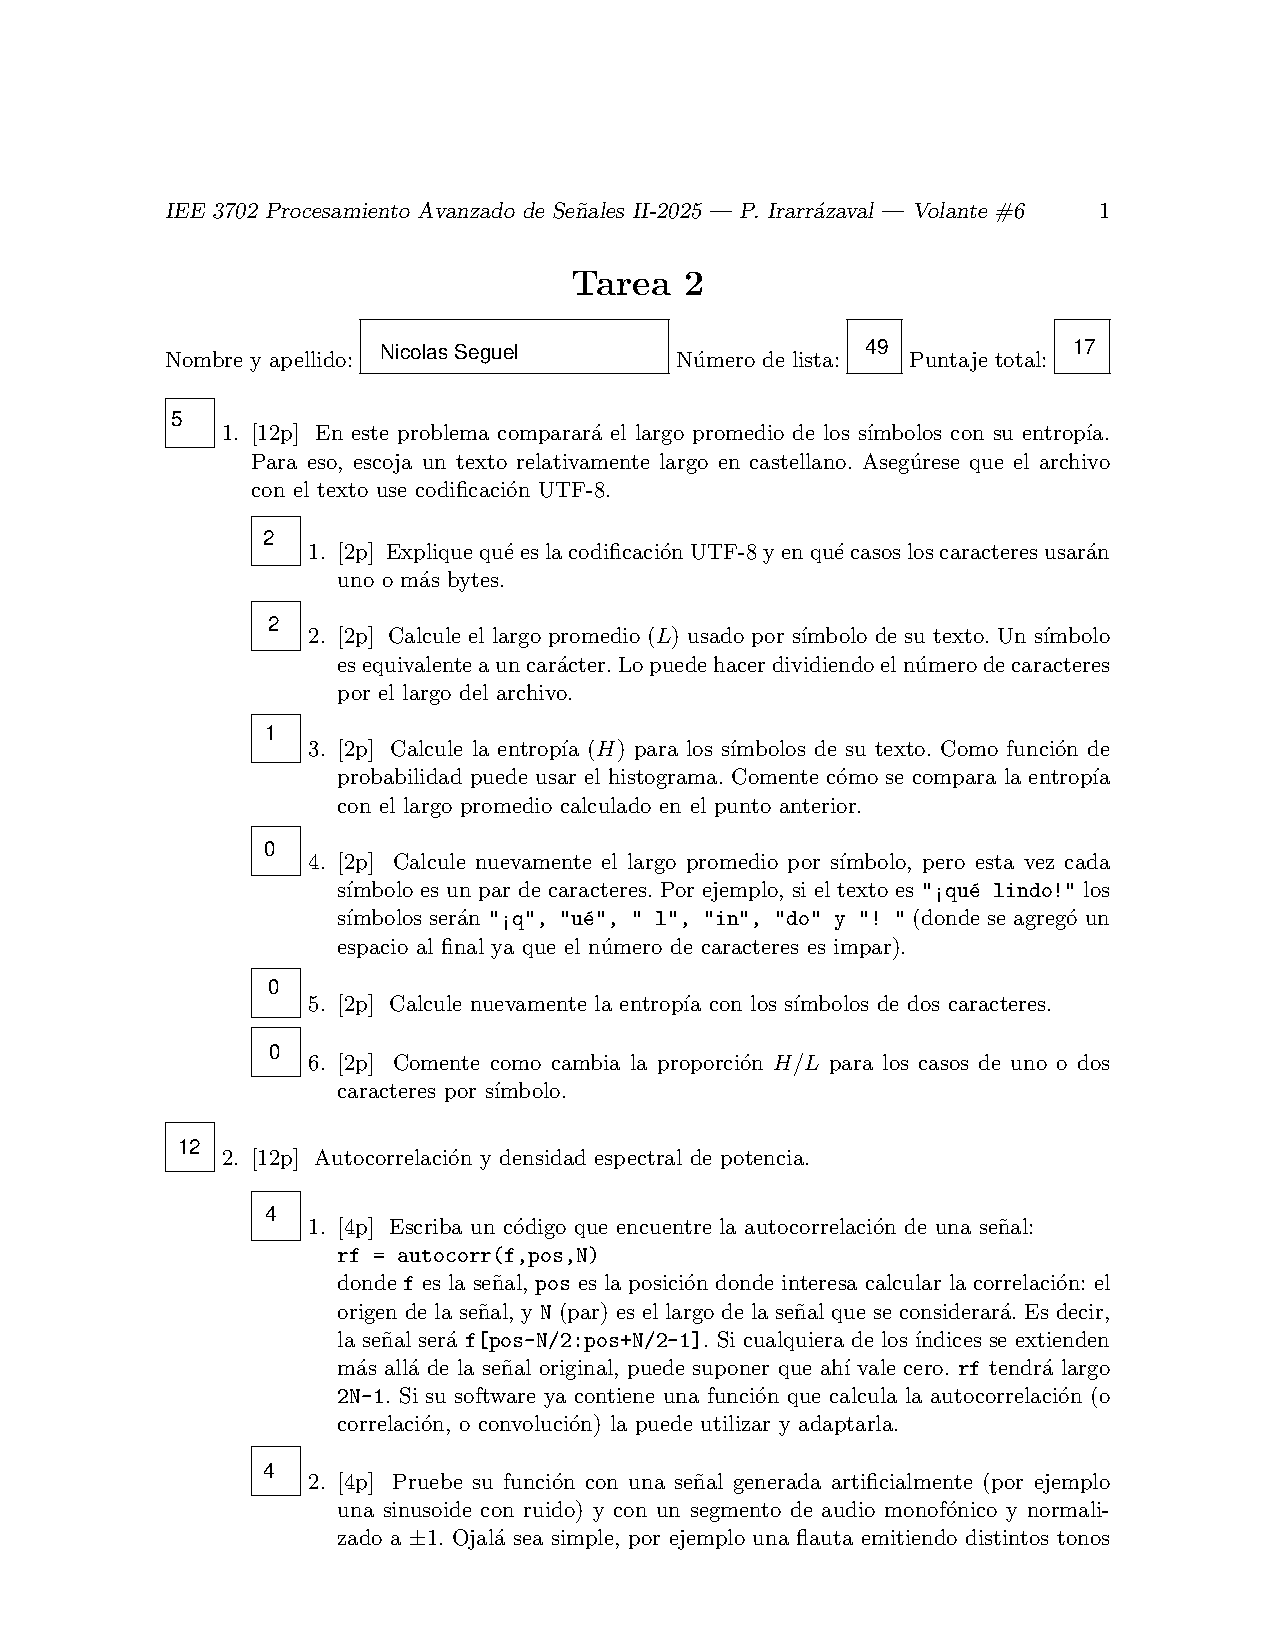
\includepdf[pages=-]{data/06.tarea02.pdf}
\maketitle

% ==== Ejemplo de respuesta con texto y fórmulas ====
\section*{Problema 1}

En este problema comparará el largo promedio de los símbolos con su entropía. Para eso, escoja un texto relativamente largo en castellano. Asegúrese que el archivo con el texto use codificación UTF-8.

\subsection*{1.1: Codificación UTF-8}

Explique qué es la codificación UTF-8 y en qué casos los caracteres usarán uno o más bytes.

\paragraph{Solución}

La codificación UTF-8 es un sistema de codificación de caracteres que permite representar texto en computadoras y otros dispositivos electrónicos. Es capaz de codificar todos los caracteres posibles en Unicode, utilizando entre uno y cuatro bytes por carácter. Los caracteres ASCII (los primeros 128 caracteres) utilizan un solo byte, mientras que los caracteres de otros idiomas o símbolos especiales utilizan más bytes.

\subsection*{1.2: Largo promedio de símbolo}

Calcule el largo promedio (L) usado por símbolo de su texto. Un símbolo es equivalente a un carácter. Lo puede hacer dividiendo el número de caracteres por el largo del archivo.

\paragraph{Solución}

El largo promedio de símbolo \( L \) se calcula como:

\[
L = \frac{N}{T}
\]

donde \( N \) es el número de caracteres y \( T \) es el tamaño del archivo en bytes.

El texto utilizado es el libro "El Principito". Tiene un total de $81516$ caracteres y $83342$ bytes. Por lo que el largo promedio de símbolo es:

\[
L = \frac{81516}{83342} \approx 0.978
\]

\lstinputlisting[language=Python, caption={Código para calcular el largo promedio de símbolo.}]{src/p1_2.py}

\subsection*{1.3: Entropía}

Calcule la entropía (H) para los símbolos de su texto. Como función de probabilidad puede usar el histograma. Comente cómo se compara la entropía con el largo promedio calculado en el punto anterior.

\paragraph{Solución}

La entropía \( H \) se puede calcular utilizando la fórmula:

\[
H = -\sum_{i} p_i \log_2(p_i)
\]

donde \( p_i \) es la probabilidad de cada símbolo en el texto. Para calcular \( p_i \), se puede usar el histograma de frecuencias de los símbolos.

\bigskip

\section*{Problema 2}

\subsection*{2.1: Implementación de la autocorrelación}

Escriba un código que encuentre la autocorrelación de una señal: \texttt{rf = autocorr(f,pos,N)} donde \textbf{f} es la señal, \textbf{pos} es la posición donde interesa calcular la correlación: el origen de la señal, y \textbf{N} (par) es el largo de la señal que se considerará. Es decir, la señal será \texttt{f[pos-N/2:pos+N/2-1]}. Si cualquiera de los índices se extienden más allá de la señal original, puede suponer que ahí vale cero. \textbf{rf} tendrá largo \texttt{2N-1}. Si su software ya contiene una función que calcula la autocorrelación (o correlación, o convolución) la puede utilizar y adaptarla.

\lstinputlisting[language=Python, caption={Código para calcular la autocorrelación.}]{src/p2_1.py}

\subsection*{2.2: Prueba de la función}

Pruebe su función con una señal generada artificialmente (por ejemplo una sinusoide con ruido) y con un segmento de audio monofónico y normalizado a ±1. Ojalá sea simple, por ejemplo una flauta emitiendo distintos tonos o la lectura de vocales. Empleando su función grafique la autocorrelación en distintas posiciones. Utilice un largo N suficientemente largo como para apreciar la forma de la autocorrelación, pero suficientemente corto para no hacer excesiva la carga computacional.

\lstinputlisting[language=Python, caption={Código para probar la autocorrelación.}]{src/p2_2.py}

\begin{figure}
    \centering
    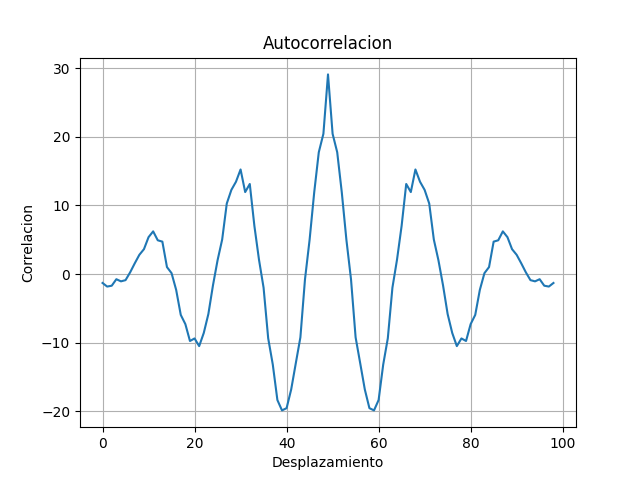
\includegraphics[width=0.8\textwidth]{figs/autocorrelacion_seno.png}
    \caption{Autocorrelación de la señal senoidal}
\end{figure}

\lstinputlisting[language=Python, caption={Código para calcular la autocorrelación.}]{src/p2_2_audio.py}

\begin{figure}[H]
    \centering
    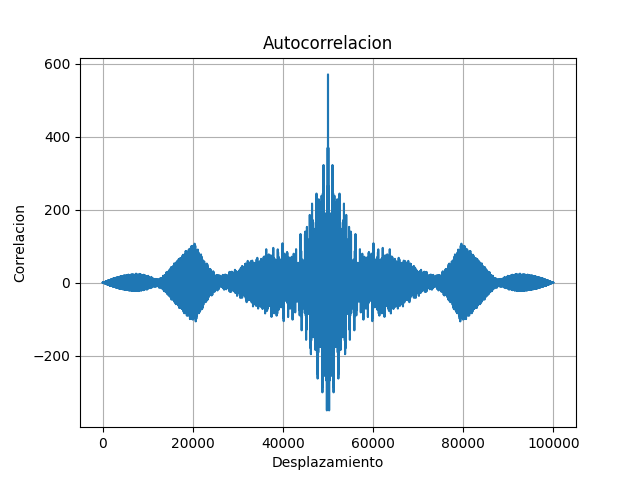
\includegraphics[width=0.8\textwidth]{figs/autocorrelacion.png}
    \caption{Autocorrelación de la señal de audio}
\end{figure}

\subsection*{2.3: Densidad espectral de potencia}

Para las mismas posiciones del punto anterior calcule y grafique la densidad espectral de potencia.

\begin{figure}
    \centering
    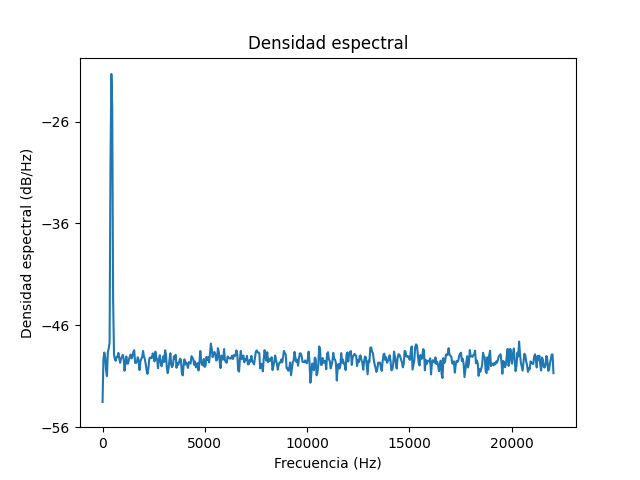
\includegraphics[width=0.8\textwidth]{figs/densidad_espectral_seno.png}
    \caption{Densidad espectral de potencia de la señal senoidal}
\end{figure}

\begin{figure}[H]
    \centering
    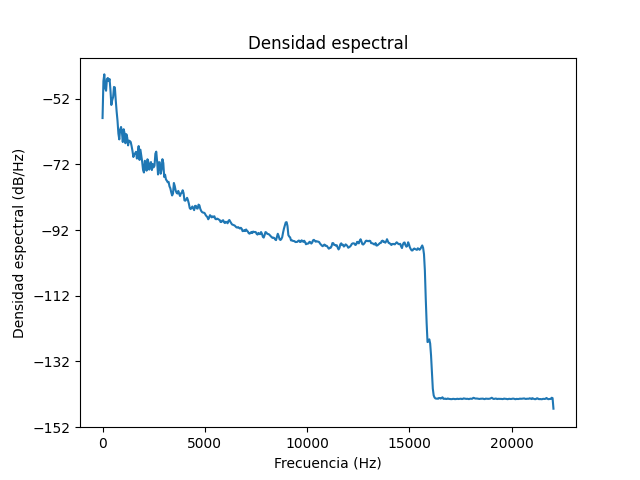
\includegraphics[width=0.8\textwidth]{figs/densidad_espectral_audio.png}
    \caption{Densidad espectral de potencia de la señal de audio}
\end{figure}

\lstinputlisting[language=Python, caption={Código para calcular la densidad espectral de potencia.}]{src/p2_3.py}

\end{document}
